
\lstset{
 language=bash,               % 设置语言为bash
 basicstyle=\ttfamily\small,  % 使用等宽字体和较小字号
 keywordstyle=\color{blue}\bfseries, % 关键字样式
 stringstyle=\color{red},     % 字符串样式
 commentstyle=\color{green!50!black}, % 注释样式
 numberstyle=\tiny,          % 行号字体大小
 numbersep=5pt,              % 行号与代码间隔
 showspaces=false,           % 不显示空格
 showstringspaces=false,     % 不强调字符串中的空格
 frame=single,               % 添加边框
 breaklines=true,            % 自动换行
 breakatwhitespace=true,     % 只在空白符处换行
 tabsize=4                   % 制表符宽度
}
\begin{CJK*}{UTF8}{song}

{\begin{CJK*}{UTF8}{zhhei}\subsection{下载与安装}\end{CJK*}}

我们的工具已经开源\footnote{
\url{https://github.com/Hepisces/db_final}}, 接下来将展示使用Anaconda进行包管理下的下载与安装流程。

\begin{figure*}
  \centering
  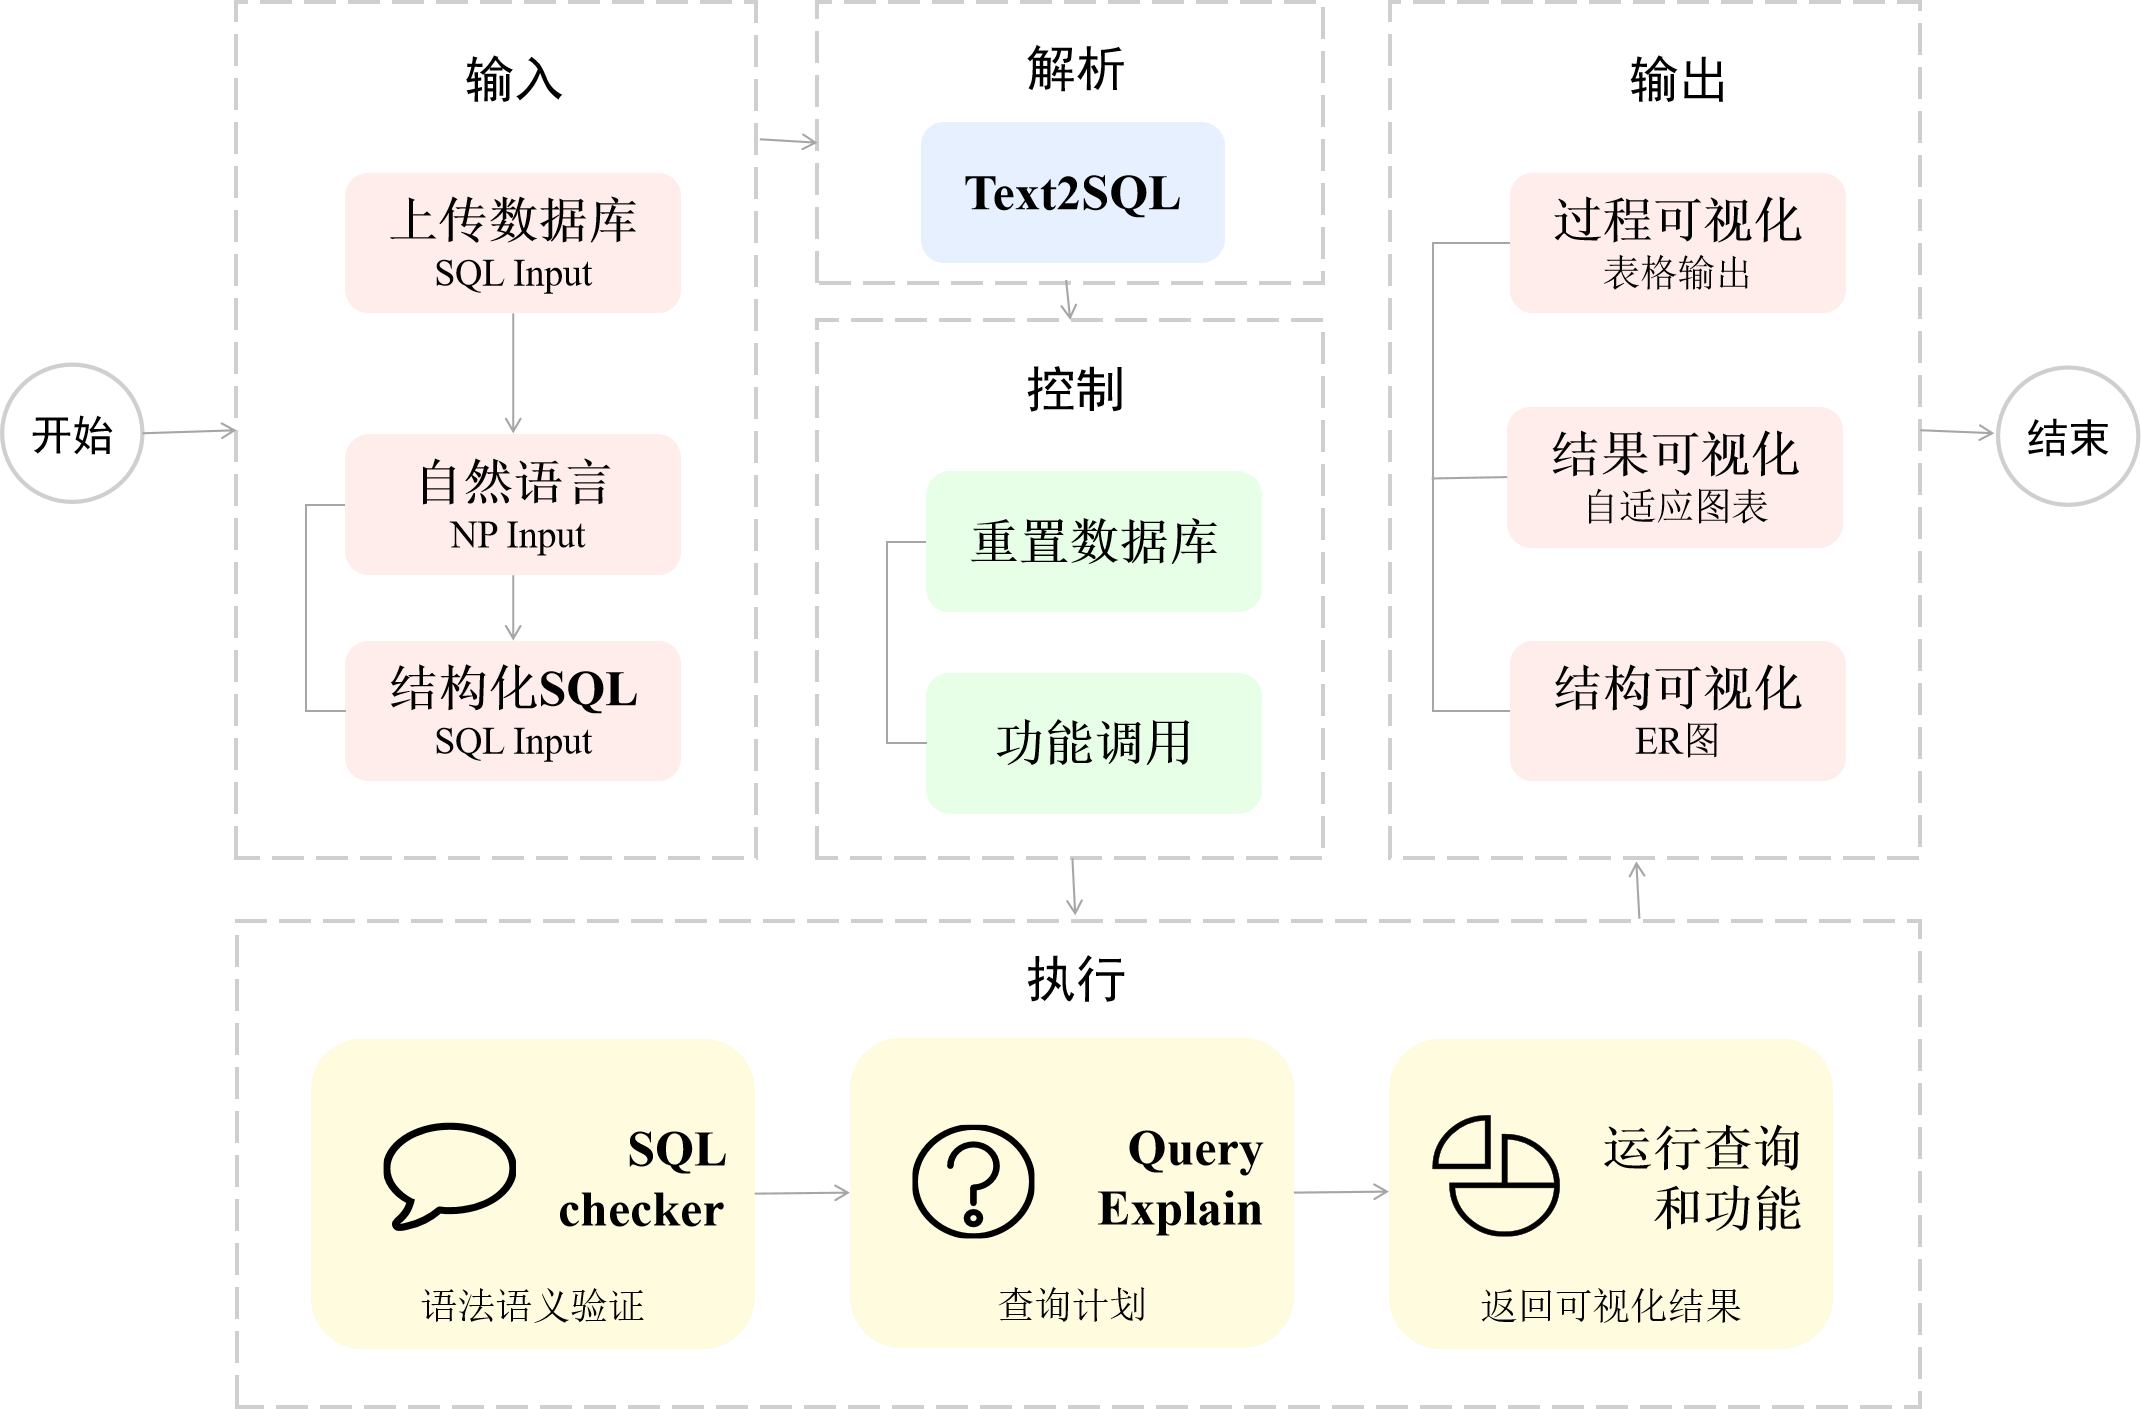
\includegraphics[width=0.9\textwidth]{article/presentation/figures/pipeline}
  \caption{架构设计}
  \label{fig:pipeline}
\end{figure*}

\begin{enumerate}
    \item 首先下载并进入文件夹

\begin{lstlisting}
> git clone \ git@github.com:Hepisces/db_final.git
> cd db_final
\end{lstlisting}

\item 使用conda创建新的虚拟环境
\begin{lstlisting}
> conda create -n awesql python=3.12 -y
> conda activate awesql
\end{lstlisting}

\item 安装相关依赖项,考虑到Text2SQL需要本地模型,下载权重耗时较长,对于简单测试并不是必须的,所以我们提供两种安装方式,当不指定AI选项时,则不会安装Text组件需要的相关库
\begin{lstlisting}
(awesql)> pip install -e .
(awesql)> pip install -e '.[AI]'
\end{lstlisting}
\end{enumerate}

{\begin{CJK*}{UTF8}{zhhei}\subsection{功能测试与效果展示}\end{CJK*}}

为了让展示的效果足够直观,我们为每个命令录制了演示视频,视频可以通过仓库的demo.md文件进行查看。\footnote{
\url{https://github.com/Hepisces/db_final/blob/main/demo.md}}

\begin{enumerate}
    \item 可以通过 help 直接展示各个使用方法

    
    \begin{lstlisting}
(awesql)> awesql --help  
    \end{lstlisting}
    
    \item 导入数据,这里假设你已经下载好了数据并且放到了db\_final的目录下
    \begin{lstlisting}
(awesql)> awesql import-data     
    \end{lstlisting}
    \item 展示当前数据库下的所有表
    \begin{lstlisting}
(awesql)> awesql tables
    \end{lstlisting}
    \item 渲染E-R图
    \begin{lstlisting}
(awesql)> awesql er
    \end{lstlisting}
        \item SQL正确性检查(示例给出的代码错误包括但不仅限于别名错误,非法字符等)
    \begin{lstlisting}
(awesql)> awesql check "SELECT STRFTIME('%Y-%m-%d', d.time) AS date, l.area, COUNT(d.did) AS update.
count, AVG(d.did) FROM devupdata d JOIN devlist | ON d.did = I.did WHERE I.area IS NOT NULL AND
STRETIME('%Y-%m-%d', d.time) > 1999-01-01' GROUP BY date, l.area ORDER BY date;"
    \end{lstlisting}
        \item 通过正确性检查后即可将代码进行查询尝试,后续即可根据交互式命令选择可视化图形类别

    \begin{lstlisting}
(awesql)> awesql run "
SELECT STRFTIME('%Y-%m-%d', d.time) AS date, l.area, COUNT(d.did) AS update_count
FROM devupdata d JOIN devlist l ON d.did = l.did 
WHERE l.area IS NOT NULL AND STRFTIME('%Y-%m-%d', d.time) > '2021-01-01' 
GROUP BY date, l.area ORDER BY date;"        
    \end{lstlisting}
        \item 使用自然语言查询(通常耗时较久,并推荐显存大于24GB的显卡使用)
    \begin{lstlisting}
(awesql)> awesql ask "Querying the time column of the devuplist table"
    \end{lstlisting}
        \item 重置数据库(这一步需要在提示以后输入管理员账户与密码)
    \begin{lstlisting}
(awesql)> awesql reset-db
    \end{lstlisting}
\end{enumerate}



\end{CJK*}